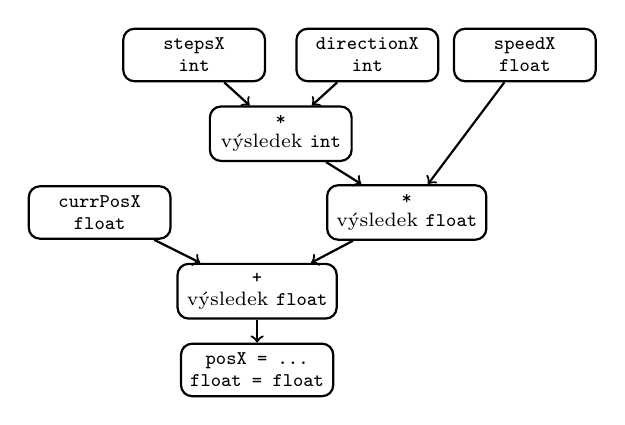
\begin{tikzpicture}[
    every node/.style={font=\scriptsize},
    box/.style={
        draw,
        rounded corners,
        thick,
        align=center,
        minimum width=1.8cm,
        minimum height=0.55cm
    },
    arrow/.style={->, thick}
]

    \node<4->[box] (a) at (0,0) {\texttt{stepsX}\\\texttt{int}};
    \node<4->[box] (b) at (2.2,0) {\texttt{directionX}\\\texttt{int}};
    \node<5->[box] (mul1) at (1.1,-1.0) {\texttt{*}\\výsledek \texttt{int}};

    \draw<5->[arrow] (a) -- (mul1);
    \draw<5->[arrow] (b) -- (mul1);

    \node<6->[box] (c) at (4.2,0) {\texttt{speedX}\\\texttt{float}};
    \node<6->[box] (mul2) at (2.7,-2.0) {\texttt{*}\\výsledek \texttt{float}};

    \draw<6->[arrow] (mul1) -- (mul2);
    \draw<6->[arrow] (c) -- (mul2);

    \node<6->[box] (d) at (-1.2,-2.0) {\texttt{currPosX}\\\texttt{float}};
    \node<7->[box] (plus) at (0.8,-3.0) {\texttt{+}\\výsledek \texttt{float}};

    \draw<7->[arrow] (d) -- (plus);
    \draw<7->[arrow] (mul2) -- (plus);

    \node<8->[box] (assign) at (0.8,-4.0) {\texttt{posX = ...}\\\texttt{float = float}};

    \draw<8->[arrow] (plus) -- (assign);

\end{tikzpicture}
